\section{Day-ahead commitment and intraday joint-recovery method}
\label{sec:method}

The proposed method couples a day-ahead commitment stage with an intraday rolling stage (\figref{fig:framework}).
On day D$-$1, a two-stage model chooses the commitments $C_k$ of all announced events, anticipating the joint recovery
between them; the capability region of \secref{sec:region} describes which commitment vectors can be delivered. On
day D, a rolling MPC re-optimises catch-up computing, storage and IES dispatch every 15~min, either centrally or by a
distributed plan--price exchange between the IT scheduler and the facility controller.

\begin{figure*}[!t]
\centering
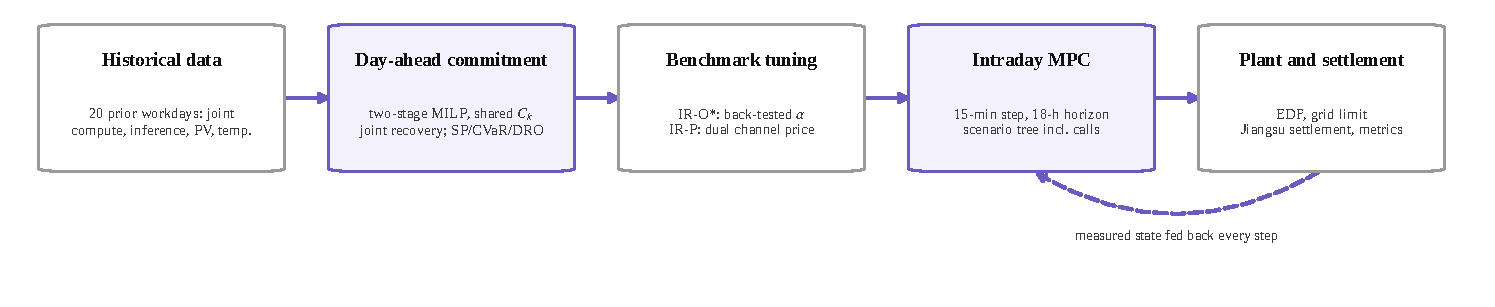
\includegraphics[width=0.98\textwidth]{fig00_framework.pdf}
\caption{Framework of the day-ahead coupled commitment and intraday joint-recovery method. The benchmarks are tuned on
the same historical data before the operating day; the measured state is fed back at every 15-min step.}
\label{fig:framework}
\end{figure*}

\subsection{Day-ahead coupled commitment and its distributionally robust reformulation}
\label{sec:dayahead}

The first-stage decision is the commitment vector $x=(C_k)_{k\in\Kset}$, shared by all scenarios; the second stage is
the joint recovery model of \secref{sec:system}--\ref{sec:model} with one set of operating variables per scenario. The
product $C_kz_{k,\omega}$ in \eqref{eq:valid} is linearised exactly by McCormick inequalities because $z_{k,\omega}$ is
binary. The base model uses five equally likely historical joint scenarios of computing load, inference, PV and
temperature, selected deterministically by load and irradiance quantiles; joint historical days preserve the
coincidence of these drivers. To hedge against an inaccurate empirical distribution, the expected cost is replaced by
its worst case over the $\ell_1$ ball (total-variation ball) around the empirical probabilities $\hat p$,
\begin{gather}
\mathcal P_\delta=\Big\{p\in\mathbb R^{|\Omega|}_{\ge0}:\ \sum_\omega p_\omega=1,\ \sum_\omega|p_\omega-\hat p_\omega|\le\delta\Big\},\nonumber\\
\min_x\ c_0(x)+\max_{p\in\mathcal P_\delta}\sum_\omega p_\omega f_\omega(x),
\label{eq:dro}
\end{gather}
where $f_\omega(x)=\min\{c_\omega^\top y_\omega:\ y_\omega\in\mathcal Y_\omega(x)\}$ is the second-stage cost of scenario
$\omega$, including the binary validity variables of the Jiangsu settlement, and $c_0(x)=-\epsilon\sum_kC_k$ is a tiny
tie-breaking value of committed capacity.

\begin{proposition}[Exact MILP reformulation of the distributionally robust commitment]\label{prop:dro}
For every $\delta\ge0$, problem \eqref{eq:dro} is equivalent to the single-level MILP
\begin{equation}
\begin{aligned}
\min_{x,\,y_\omega,\,\eta,\,\lambda,\,\nu}\ & c_0(x)+\eta+\sum_\omega\hat p_\omega\lambda_\omega+\delta\nu\\
\text{s.t.}\ & c_\omega^\top y_\omega\le\eta+\lambda_\omega,\quad -\nu\le\lambda_\omega\le\nu\qquad\forall\omega\in\Omega,\\
& y_\omega\in\mathcal Y_\omega(x)\quad\forall\omega\in\Omega,\qquad \nu\ge0.
\end{aligned}
\label{eq:droR}
\end{equation}
Moreover, $\delta=0$ yields the two-stage stochastic programme (SP) and $\delta\ge2(1-\min_\omega\hat p_\omega)$ the
scenario-robust problem (RO); for fixed $x$ the worst-case distribution moves the probability mass
$\min\{\delta/2,\,1-\hat p_{\bar\omega}\}$ from the cheapest scenarios to the most expensive scenario $\bar\omega$; and the
optimal value $V(\delta)$ is non-decreasing and concave in $\delta$, with $\nu^*$ a supergradient, \ie\ the marginal
price of robustness.
\end{proposition}

Problem \eqref{eq:droR} adds only $2|\Omega|+1$ continuous variables and $3|\Omega|$ constraints and keeps the binaries
of the second stage, so no semidefinite reformulation or column-and-constraint generation~\cite{zhang2026bilevel,zeng2013}
is needed, which would not be exact with binary recourse. In the same way, $\mathrm{CVaR}_\beta$ and mean--CVaR
objectives are linearised by the Rockafellar--Uryasev formula~\cite{rockafellar2000}. When an event is uncertain, it
appears only in $\mathrm{round}(p_kS)$ of the $S$ scenarios, spread evenly over the load quantiles. As an alternative
scenario generator, all $20\times14=280$ pairs of historical computing days and weather days are clustered by K-means (farthest-point
initialisation, Lloyd iterations) on standardised 12--24~h hourly profiles of deferrable GPUs, inference GPUs and
renewable output (plus the chiller COP in the seasonal-drift test); the medoid of each cluster becomes a scenario and
the cluster share its, generally non-uniform, probability, around which the $\ell_1$ ball is built.

\subsection{Deliverable capability region of commitment vectors}
\label{sec:region}

A single commitment value per event is the current bidding format, but what the data center can actually offer is a
set of commitment vectors. Let all $K$ events with fixed times be called. A vector $C=(C_1,\dots,C_K)\ge0$ is
deliverable if some operation that meets all deadlines and the connection limit achieves a mean reduction of at least
$C_k$ in every event, \ie\ full delivery without shortfall. Denote by $\Cset$ the set of deliverable vectors under
joint recovery (the capability region), by $\Cset_\Pi$ the set under a sequential strategy $\Pi$ (IR-O, IR-O*, IR-P),
and by $\Gamma^0_k$ the stand-alone capability of event $k$.

\begin{proposition}[Capability region and virtual-battery description]\label{prop:region}
(i) $\Cset$ is a bounded convex polytope that is downward closed and contained in the single-event box
$\mathcal B=\prod_k[0,\Gamma^0_k]$. (ii) $\Cset_\Pi\subseteq\Cset$ for every sequential strategy $\Pi$. (iii) For every
block $S=\{i,\dots,j\}$ of consecutive events,
\begin{equation}
\sum_{k\in S}D_kC_k\le\bar b_S:=\bar X(e_j)+E_s^{\max}+H_S+g\,D_S+\Delta_S ,
\label{eq:multibound}
\end{equation}
where $\bar X(e_j)$ is the virtual-storage capacity at the end of the block, $E_s^{\max}$ the dischargeable energy of
full storage, $H_S$ the channel energy of the gaps in the block, $gD_S$ the gas-engine headroom during the events, and
$\Delta_S=\sum_{t\in\Tset_S}(\Pb_t-P^{\mathrm{nom}}_t)\dt$ the difference between the baseline and the same-day import
without response; no unbiased-baseline assumption is needed. Hence $\Cset\subseteq\mathcal V:=\mathcal B\cap\{\sum_{k\in
S}D_kC_k\le\bar b_S\}$, a virtual battery with event power limits $\Gamma^0_k$ that is recharged in the gaps at the
channel width. (iv) Let $h_S=\max\{\sum_{k\in S}D_kC_k:C\in\Cset\}$ and $\mathcal T=\mathcal B\cap\{\sum_{k\in S}D_kC_k\le
h_S,\ |S|\ge2\}$. Then $\theta^*\mathcal T\subseteq\Cset\subseteq\mathcal T$ with $\theta^*=\min_v\min\{1,\theta_v\}$,
$\theta_v=\max\{\theta:\theta v\in\Cset\}$ over the vertices $v$ of $\mathcal T$; $\theta^*=1$ certifies
$\Cset=\mathcal T$. (v) For price coordination, $\Cset_{\mathrm{IR\text{-}P}}\subseteq\Cset_{\mathrm{IR\text{-}P+}}\subseteq\Cset$,
where IR-P+ denotes delivery with the most favourable optimal IT response to the channel price, which a single
combined LP decides.
\end{proposition}

Part (iv) gives a verifiable inner approximation with one LP per support value and per vertex. If $\mathcal V$ or
$\mathcal T$ describes $\Cset$, the data center can bid the event power limits $\Gamma^0_k$ and a few cross-event energy
budgets ($K+1$ numbers in the case study) and the grid operator may call any combination within them. Part (v) reveals
that the response of the IT side to a given channel price is not unique, so a price alone does not determine a
deliverable plan; this motivates the plan--price exchange of \secref{sec:admm}.

\subsection{Intraday rolling joint recovery}
\label{sec:mpc}

On day D, the MPC is re-solved every 15~min over an 18-h horizon (72 steps). The deterministic MPC (JR-D) uses the
historical mean forecast corrected by the error of the last hour; the scenario MPC (JR-S) uses five scenarios with a
non-anticipative first step~\cite{schildbach2014}. Before an uncertain event is confirmed, JR-S represents it by a
scenario tree (the event occurs in three of the five scenarios), whereas the deterministic strategies use the certainty
equivalent (an event with probability of at least 0.5 is treated as called); after confirmation all strategies use the
true state. The terminal storage references come from the day-ahead plan, the settlement of events that are under way
uses the reduction already accrued, and the planner falls back to the rule-based strategy if a solve fails. Within each class, the executed GPUs are assigned to jobs by EDF, which by Lemma~\ref{lem:edf} meets every
deadline.

\subsection{Distributed implementation by plan--price exchange}
\label{sec:admm}

Joint recovery does not require merging the IT scheduler and the facility controller. With the binaries fixed (every
called event valid), the joint model is an LP whose variables split into the IT side $x_{\mathrm{IT}}$ (job execution,
backlog, capping, overheads; cost $f_{\mathrm{IT}}$: delay, overdue and terminal backlog value) and the facility side
$x_{\mathrm F}$ (grid, PV, gas engine, chillers, BESS, TES, settlement; cost $f_{\mathrm F}$). They are coupled only by
the deferrable dynamic IT power $p_t=\pdyn\sum_c(y_{c,t}-\zeta_{c,t})$, one number per step, which appears in
\eqref{eq:cool} and \eqref{eq:elec}; let $q_t$ be the facility's copy. With a price vector $\lambda$ and a penalty
$\rho>0$, the two sides iterate (ADMM~\cite{boyd2011})
\begin{equation}
\begin{aligned}
x_{\mathrm{IT}}^{k+1}&=\arg\min\ f_{\mathrm{IT}}+\lambda^{k\top}p+\tfrac{\rho}{2}\|p-q^k\|^2,\\
x_{\mathrm F}^{k+1}&=\arg\min\ f_{\mathrm F}-\lambda^{k\top}q+\tfrac{\rho}{2}\|q-p^{k+1}\|^2,\\
\lambda^{k+1}&=\lambda^k+\rho\big(p^{k+1}-q^{k+1}\big),
\end{aligned}
\label{eq:admm}
\end{equation}
exchanging only the plans $p^{k+1}$, $q^{k+1}$; the price is updated by both sides with the same formula, and neither
side needs the other's model, state or forecast.

\begin{proposition}[Distributed joint recovery]\label{prop:admm}
(i) The joint model is equivalent to $\min_pF_{\mathrm{IT}}(p)+F_{\mathrm F}(p)$, where both value functions are convex
and piecewise linear. (ii) For every $\rho>0$, the residual $p^k-q^k\to0$, the total cost converges to the joint
optimum and $\lambda^k$ converges to an optimal dual $\lambda^*$ of the coupling. (iii) If the electric chiller is
interior at step $t$, $\lambda^*_t=\varphi_t\dt\,\lch_t$ with $\varphi_t=1+a^{\mathrm{aux}}+\theta/\COP_t$, where
$\lch_t$ is the channel price of Proposition~\ref{prop:price}: the iteration discovers the channel price. (iv) The
quadratic terms make each side's response unique and thereby select a mutually compatible pair among the many optimal
responses to a fixed price.
\end{proposition}

Because glpk cannot solve quadratic programmes, the price term is kept exact and only the proximal term is
approximated by tangent cuts centred at the other side's latest plan, with tangent points densest near zero deviation
($\pm$0.005 to $\pm$20~MW); the approximation error is at most $\rho\delta_p^2/8$ for a tangent spacing $\delta_p$,
and both subproblems remain LPs. In closed loop, JR-A performs $K$ iterations (1--10) per MPC step, warm-started from
the previous step's price and facility plan; any remaining mismatch is absorbed by the grid import.

\subsection{Algorithm flow and computational efficiency}
\label{sec:algorithm}

The complete procedure is summarised in \tabref{tab:algorithm}. Each MPC step solves one MILP whose number of binaries
is the number of remaining events times the number of scenarios (at most 3 for JR-D and 15 for JR-S).
\tabref{tab:timing} reports the model size and median solve time with single-threaded GNU Octave 8.4 and glpk on an
idle machine (experiment~14). Even the 10-scenario MPC solves in less than 2~s, far below the 15-min control interval,
and the deterministic MPC simulates a whole day (120 steps) in about 4~s. The size grows linearly with the number of
scenarios. The day-ahead SP solves in at most 4.3~s and the distributionally robust commitment with ten scenarios in
14--25~s, both as single MILPs, whereas the moment-based DRO planning model of~\cite{zhang2026bilevel} needs eight
column-and-constraint generation iterations and about 850~s.

\begin{table}[!t]
\caption{Algorithm 1: day-ahead coupled commitment and intraday joint-recovery MPC.}
\label{tab:algorithm}
\centering
\fontsize{7.1}{8.7}\selectfont
\begin{tabularx}{\columnwidth}{@{}X@{}}
\toprule
\textbf{Input:} historical day pool $\{\xi_\omega\}$; event notices $(s_k,e_k,\pi_k,p_k$, notice times$)$; baseline
$\Pb$; parameters; risk setting (SP, $\mathrm{CVaR}_\beta$ or DRO $\delta$).\\
\textbf{Output:} commitments $C_k$; 15-min set-points; Jiangsu settlement.\\
\midrule
\textit{Day-ahead (D$-$1)}
\algline{1}{Select $S$ joint scenarios by quantiles (or K-means medoids) with probabilities $\hat p_\omega$; an event with
call probability $p_k<1$ appears in $\mathrm{round}(p_kS)$ scenarios.}
\algline{2}{Solve the two-stage MILP: first stage $C_k$, second stage the joint recovery model per scenario,
$C_kz_{k,\omega}$ linearised by McCormick, risk measure by Proposition~\ref{prop:dro}.}
\algline{3}{Declare $C_k$; store the terminal references $E^{\mathrm{ref}}$, $S^{\mathrm{ref}}$; tune the
benchmarks ($\alpha^*$, IR-P price) on the same data.}
\textit{Intraday (day D, every step $t=1,\dots,T$)}
\algline{4}{Measure the state: backlog per class and deadline, $E_t$, $S_t$, reductions and rebound accrued.}
\algline{5}{Correct the forecasts by the last-hour error; update event calls at confirmation times.}
\algline{6}{Build the $\min(72,T-t+1)$-step joint model: JR-D with the certainty-equivalent events, JR-S with $S$
scenarios and a non-anticipative first step; embed the remaining settlement, rebound windows, lag bounds
\eqref{eq:lag} and terminal values \eqref{eq:term}.}
\algline{7}{Solve the MILP (JR-A: $K$ plan--price iterations \eqref{eq:admm}); on failure fall back to IR-R.}
\algline{8}{Apply the first step: GPUs per class (EDF within the class) and storage/IES set-points; the facility keeps
$\Pg_t\le\Pcap$ by storage first.}
\algline{9}{Record and move to $t+1$.}
\textit{Settlement (end of day D)}
\algline{10}{Settle every event by the Jiangsu rules and compute all indicators of \tabref{tab:metrics}.}\\
\bottomrule
\end{tabularx}
\end{table}

\begin{table}[!t]
\caption{Model size and solve time (median, single-threaded Octave 8.4 with glpk; $T$: horizon in 15-min steps,
$S$: scenarios, $K$: events).}
\label{tab:timing}
\centering\footnotesize
\setlength{\tabcolsep}{3.2pt}
\begin{tabular}{@{}lrrrrrrr@{}}
\toprule
Model & $T$ & $S$ & $K$ & Variables & Binaries & Constraints & Time (s)\\
\midrule
Intraday MPC & 24 & 1 & 3 & 520 & 3 & 392 & 0.007\\
Intraday MPC (JR-D) & 72 & 1 & 3 & 1,193 & 3 & 880 & 0.029\\
Intraday MPC & 72 & 5 & 3 & 5,965 & 15 & 4,444 & 0.48\\
Intraday MPC & 72 & 10 & 3 & 11,930 & 30 & 8,899 & 1.91\\
Intraday MPC & 72 & 5 & 2 & 5,940 & 10 & 4,384 & 0.46\\
Intraday MPC & 72 & 5 & 4 & 5,990 & 20 & 4,504 & 0.49\\
Day-ahead SP & 120 & 5 & 2 & -- & -- & -- & 2.25\\
Day-ahead SP & 120 & 5 & 3 & -- & -- & -- & 2.87\\
Day-ahead SP & 120 & 5 & 4 & -- & -- & -- & 4.32\\
Day-ahead DRO & 120 & 10 & 3 & -- & 30 & -- & 14--25\\
\bottomrule
\end{tabular}
\end{table}
